\documentclass[a4paper,11pt]{article}
\usepackage[T1]{fontenc}
\usepackage[utf8]{inputenc}
\usepackage{lmodern}
\usepackage{ngerman}
\usepackage{amsmath}
\usepackage{graphicx}
\usepackage{pdfpages}
\usepackage{siunitx}
\usepackage{kpfonts}



\setcounter{secnumdepth}{0}
\title{Übungsblatt 2}
\author{Lennard Behrens (3200335), Gabriel Kraus (3208414)}

\begin{document}

\maketitle

\section*{Aufgabe 1}
Die maximale Flughöhe während des Parabelflugs sei $x_1$ und die ursprüngliche Flughöhe sei $x_0$. Zum Zeitpunkt $t=0$ hat das Flugzeug den Scheitelpunkt der Parabelbahn erreicht. Allgemein gilt für die Flughöhe $x$
\begin{align*}
  x(t) = x_1 + v_xt- \frac{1}{2} g t^2
\end{align*} 
Zum Zeitpunkt $t_0$ hat das Flugzeug eine Geschwindigkeit in x-Rightung $v_x=0$. Nach $\Delta t = 20 \mbox{s}$ ist das Flugzeug von Hochpunkt zurück auf die ursprüngliche Höhe gefallen. 
\begin{align*}
  x_0 &= x_1 - \frac{1}{2} g (\Delta t)^2 \\
  x_1 - x_0 &= \frac{1}{2} g (\Delta t)^2 \\
  &= 1962 \mbox{m}
\end{align*}

\section*{Aufgabe 2}
\subsection*{Aufgabe 2a}
Seien $v_0$ die Abschussgeschwindigkeit und $\alpha$ der Abschusswinkel. So gilt für die Komponenten von $v_0$
\begin{align*}
  v_{0x} &= v_0 \cdot \cos\alpha\\
  v_{0y} &= v_0 \cdot \sin\alpha \mbox{.}
\end{align*}
Daraus folgt 
\begin{align*}
  x &= t \cdot v_0 \cos\alpha \\
  y &= t \cdot v_0 \sin\alpha - \frac{1}{2}g \cdot t^2 \\
  \Rightarrow t &= \frac{x}{v_0 \cos\alpha} \mbox{.}
\end{align*}
Nun kann man $t$ eliminieren.
\begin{align*}
  y(\alpha) &= x \cdot\tan\alpha - \frac{g \cdot x^2}{2v_0^2\cdot\cos^2\alpha} \\
  &= x \cdot\left(\tan\alpha - \frac{g \cdot x}{2v_0^2\cdot\cos^2\alpha}\right)
\end{align*}
Nun bestimmt man die Nullstellen dieser Funktion $y(\alpha)$, um die zurückgelegte Distanz zu erhalten.
\begin{align*}
  y(\alpha) &= x\cdot\left(\tan\alpha - \frac{g \cdot x}{2v_0^2\cdot\cos^2\alpha}\right) \\
  \Rightarrow x_1 &= 0 \\
  0 &=\tan\alpha - \frac{g \cdot x}{2v_0^2\cdot\cos^2\alpha} \\
  x_2(\alpha) &= 2\frac{v_0^2}{g} \cdot\tan\alpha\cos^2\alpha
\end{align*}
Da $x_1=0$ gibt $x_2(\alpha)$ die maximale Schussentfernung an. Um das Maximum für $x_2(\alpha)$ zu ermittelt, setzt man 
\begin{align*}
  \frac{dx_2}{d\alpha} &= 0\\
  0 &= 2\frac{v_0^2}{g}\cdot\left(1 - 2\cos\alpha\sin\alpha\tan\alpha\right)\\
  &= 2\frac{v_0^2}{g} \cdot\left(1 - 2\cdot\sin^2\alpha\right)\\
  1 &= 2\cdot\sin^2\alpha \\
  \alpha &= \arcsin\sqrt{\frac{1}{2}} = \frac{\pi}{4}=45^\circ
\end{align*}

\subsection*{Aufgabe 2b}
Aus Aufgabe 2a folgt für die Schussentfernung $d$
\begin{align*}
  d = 2\frac{v_0^2}{g} \cos^2\alpha\tan\alpha
\end{align*}
Da $\alpha = \frac{\pi}{4}$ gilt 
\begin{align*}
  d &= 2\frac{v_0^2}{g} \cos^2\alpha\\
  v_0 &= \sqrt{\frac{d\cdot g}{\cos^2\alpha}} = 28,014 \mbox{m/s}
\end{align*}

\subsection*{Aufgabe 2c}
Für die mittlere Geschwindigkeit gilt
\begin{align*}
  \overline{v} = \frac{\Delta x}{\Delta t} \Rightarrow t = \frac{\Delta x}{\overline{v}}
\end{align*}
Zu Beginn des Abbremsens hat der Ball die Geschwindigkeit $v = v_0$ und zum Ende $v = 0$. Daraus ergibt sich näherungsweise die mittlere Geschwindigkeit während des gesamten Bremsvorgangs
\begin{align*}
  \overline{v} = \frac{1}{2} v_0 \mbox{.}
\end{align*}
Daraus folgt
\begin{align*}
  \Delta t = \frac{\Delta x}{\overline{v}} = 2\frac{\Delta x}{v_0} = 3,6 \mbox{ms.}
\end{align*}

\subsection*{Aufgabe 2d}
Für die mittlere Beschleunigung gilt
\begin{align*}
  \overline{a} = \frac{\Delta v}{\Delta t}
\end{align*}
Da die Geschwindigkeit $v_0$ gänzlich aufgehoben wird, gilt
\begin{align*}
  \overline{a} = \frac{v_0}{\Delta t} = \frac{v_0^2}{2\cdot\Delta x} = 7,8\cdot 10^3 \mbox{m/s}^2\mbox{.}
\end{align*}


\section*{Aufgabe 3}
    \subsubsection*{Aufgabe 3a}
        Um den Winkel $\alpha$ berechenen, stellt man die Funktion für $z_{(t)}$ nach $\alpha$ um und setzt einen gegebenen Punkt ein, in diesem Fall ist der Punkt der, wo der Ball auf den Boden trifft.
        \begin{align*}
          h_{(t)}&=h_0+v_{h0}t-\frac{1}{2}gt^2 \\
        \end{align*}
        Im Auftreffpunkt ist t:
        \begin{align*}
          t=\frac{s}{t}=\frac{\frac{L}{2}+a}{v_x}
        \end{align*}
        Für diesen $t$-Wert ist der $y$-Wert 0.
        \begin{align*}
          0=h_0+v_{y0}t-\frac{1}{2}g\left(\frac{\frac{L}{2}+a}{v_x}\right)^2
        \end{align*}
        Einsetzen der Näherungen:
        \begin{align*}
          0=h_0+v_0\alpha t-\frac{1}{2}g\left(\frac{\frac{L}{2}+a}{v_0}\right)^2
        \end{align*}
        Nach $\alpha$ aufgelöst:
         \begin{align*}
          \alpha &= \frac{\frac{1}{2}g\left(\frac{\frac{L}{2}+a}{v_0}\right)-h_0}{\left(\frac{L}{2}+a\right)} \\
          \alpha &= -0.1295 rad = \ang{-7.41996}
        \end{align*}
        J.I. muss den Winkel \ang{-7.41996} wählen, damit der Ball nach dem Aufschlag im Punkt A auftrifft.
      \subsubsection*{Aufgabe 3b}
        Diese Aufgabe kann analog zu $a)$ gelöst werden mit dem Unterschied, dass der Punkt nicht $A$ sodern die obere Kante des Netzes sein muss.
        \begin{align*}
          t=\frac{s}{t}=\frac{\frac{L}{2}}{v_x}
        \end{align*}
        Nun in $y_{(t)}$ einsetzen und wieder mit Hilfe der Näherungen nach $\alpha$ auflösen.
        \begin{align*}
          \alpha &= \frac{h-\frac{1}{2}g\left(\frac{\frac{L}{2}}{v_0}\right)^2-h_0}{\frac{L}{2}} \\
          \alpha &= -0.1624 \mbox{rad } = \ang{-9.3056}
        \end{align*}
        Damit der Ball übers Netz fliegt muss der Winkel mind. $\ang{-9.3056}$ sein.
      \subsubsection*{Aufgabe 3c}
        \begin{align*}
          t=\frac{s}{v}=\frac{L}{v_x}\approx\frac{L}{v_0}=0.3382s
        \end{align*}
        B.T. bleiben ab dem Aufschlag $0.3382s$ bis er den Ball zurückzuschlagen muss.
\section*{Aufgabe 4}
  \subsubsection*{Aufgabe 4a}
    \begin{align*}
      \cos(\phi)&=\frac{\vert\vec{a_b}\vert}{\vert\vec{a}\vert} \\
      \cos\left(\frac{\pi}{4}\right)*\frac{5}{2}&=\frac{5\sqrt{2}}{4}
    \end{align*}
    
  \subsubsection*{Aufgabe 4b}
    \begin{align*}
      P_1&=(1,1) \quad P_2=(5,4) \quad P_3=(3,-5) \\
      \vec{a}&=\overrightarrow{P_1P_2}=\begin{pmatrix}4\\3\end{pmatrix} \quad \vec{b}=\overrightarrow{P_1P_3}=\begin{pmatrix}2\\-6\end{pmatrix} \\
      \overrightarrow{OP_4}&=\overrightarrow{OP_1}+\vec{a}+\vec{b}=\begin{pmatrix}7\\-2\end{pmatrix} \\
      P_4&=(7,-2)
    \end{align*}
    
  \subsubsection*{Aufgabe 4c}
    2 Vektoren sind zueinander senkrecht, wenn ihr Skalarprodukt 0 ergibt.
    \begin{align*}
      i) \quad&\vec{a}\cdot\vec{b}=\begin{pmatrix}2\\-3\\1\end{pmatrix}\cdot\begin{pmatrix}-1\\4\\2\end{pmatrix}(-2-12+2)=-12\neq0 \\
      ii) \quad&\vec{a}\cdot\vec{b}=\begin{pmatrix}4\\-3\\1\end{pmatrix}\cdot\begin{pmatrix}-2\\-4\\-4\end{pmatrix}(-8+12-4)=0
    \end{align*}
    Die Vektoren in $ii)$ sind senkrecht zueinander, die in $i)$ sind es nicht.
  \subsubsection*{Aufgabe 4d}
    \begin{align*}
      \cos(\varphi)&=\frac{\vec{a}\cdot\vec{b}}{\vert\vec{a}\vert\cdot\vert\vec{b}\vert}=\frac{2}{3} \\
      \varphi &= \arccos\left(\frac{2}{3}\right)=0.841rad=\ang{48.1897}
    \end{align*}
  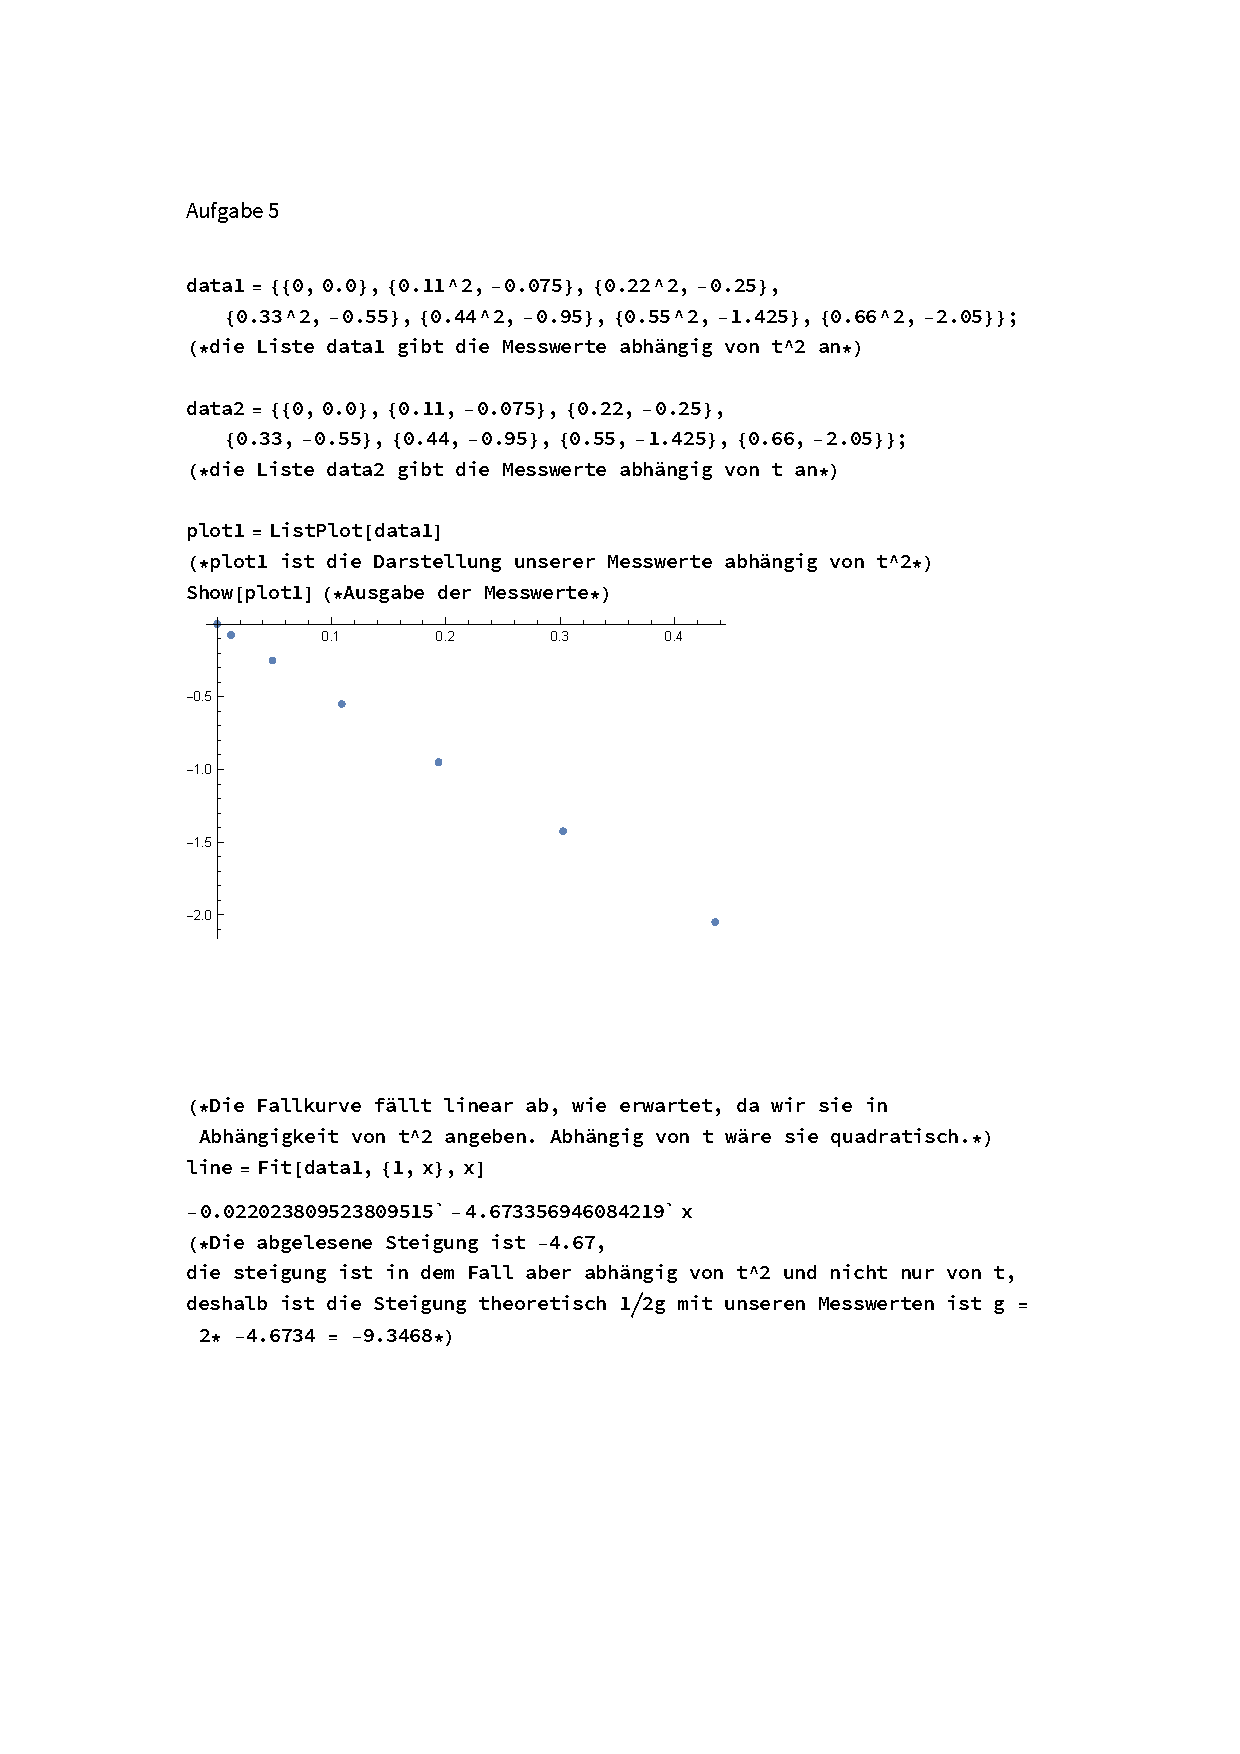
\includepdf[pages=-]{aufgabe_5.pdf}
\end{document}
